\section{Series de precipitación y caudal}

Se analiza la cuenca del río La Vieja hasta la estación Cartago (IDEAM 26127040), con un área CAMELS de 2797,19~km$^2$. El periodo comprende enero de 1981 a diciembre de 2022. Se utiliza precipitación CHIRPS v2 promediada sobre la cuenca y caudal observado según el depósito \href{https://doi.org/10.5281/zenodo.18794895}{CAMELS-COL}.

Para mantener una notación explícita, $P_{L,m}$ es la precipitación de referencia elegida: CHIRPS v2 diario, promediado sobre la cuenca por CAMELS-COL y acumulado a mm/mes. CHIRPS es un producto combinado espacial, no la observación independiente de un único pluviómetro local. $P_{I,m}$ es IMERG Final Run V07 en mm/mes. Para la comparación simultánea de $P_{L,m}$, $P_{I,m}$ y Q se define enero de 1998--diciembre de 2022, con 285 meses completos; los 15 meses sin Q se mantienen como faltantes y no se rellenan.

\subsection{Agregación y tratamiento de faltantes}
La precipitación mensual se obtiene sumando los valores diarios y el caudal mensual promediándolos. Para un mes completo con $n_m$ días:
\[
P_m=\sum_{d\in m}P_d\quad[\mathrm{mm/mes}],\qquad
Q_m=\frac{1}{n_m}\sum_{d\in m}Q_d\quad[\mathrm{m^3/s}].
\]
Se conserva únicamente un mes con el 100\,\% de sus días válidos. El calendario contiene 15\,340 días esperados y 255 ausentes (1,66\,\%). Quedan 485 meses completos de 504; los 19 restantes se mantienen como vacíos. No se rellenan ni prorratean registros y se conservan los extremos.

\begin{figure}[H]
\centering
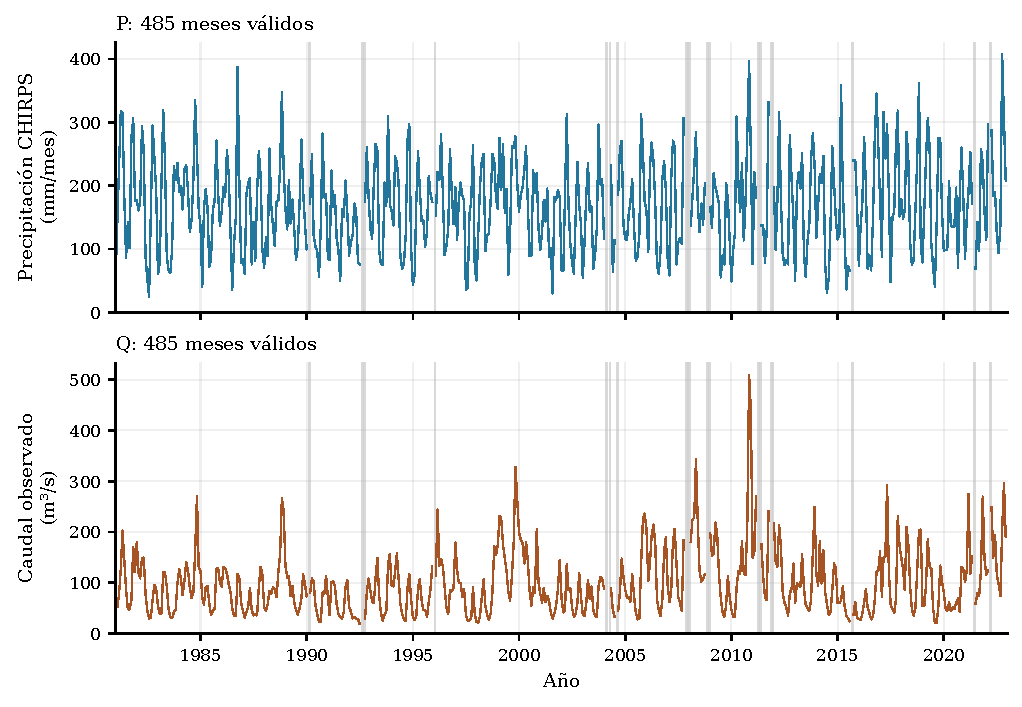
\includegraphics[width=\linewidth]{figuras/series_mensuales.pdf}
\caption{Precipitación acumulada y caudal medio mensuales de La Vieja--Cartago. Los paneles comparten el eje temporal; las franjas grises indican meses excluidos por días faltantes. Elaboración propia con CAMELS-COL.}
\label{fig:series-mensuales}
\end{figure}

\subsection{Lectura inicial y alcance}
Se observan oscilaciones estacionales y diferencias entre años (figura~\ref{fig:series-mensuales}). El máximo de precipitación mensual ocurre en octubre de 2022 (407,57~mm); el máximo de caudal medio mensual, en noviembre de 2010 (508,77~m$^3$/s). No coinciden, lo que motiva examinar los aportes previos y la respuesta de la cuenca sin atribuir todavía una causa.

\subsection{Meses extremos y contraste cronológico}
Los extremos que deben localizarse en la figura~\ref{fig:series-mensuales} son: agosto de 1982, mínimo de P (24,89~mm); octubre de 2022, máximo de P (407,57~mm); julio de 1992, mínimo de Q (18,37~m$^3$/s) y R (17,59~mm); y noviembre de 2010, máximo de Q (508,77~m$^3$/s) y R (471,45~mm). R es una conversión del caudal a lámina mensual, por lo cual sus extremos son coherentes con los de Q.

Que el máximo de P y el de Q ocurran en meses distintos no indica por sí solo un error: el caudal integra lluvia antecedente, almacenamiento y respuesta de la cuenca. Noviembre de 2010 es un episodio plausible: IDEAM documentó una temporada lluviosa inusitada durante La Niña, con humedad del suelo superior a la usual e inundaciones en las regiones Andina y del Cauca. Los mínimos de 1982 y 1992 también son compatibles con periodos secos asociados a El Niño reportados por IDEAM. Esta interpretación es de plausibilidad, no de causalidad: aún se deben revisar datos diarios, metadatos y cambios de instrumento para descartar un problema de medición.

\subsection{Referencias del contraste climático}
IDEAM (2010). \textit{Boletín diciembre de 2010}. Disponible en \url{https://www.ideam.gov.co/file-download/download/public/6150}.

IDEAM (2006). \textit{La sequía en Colombia}, nota técnica NT\_IDEAM-2006-004.

Esta primera sección presenta las series históricas y la comparación IMERG disponible desde 1998. Las gráficas no demuestran por sí solas tendencias ni causas físicas. El código Python genera la figura vectorial y una versión Plotly con las mismas fechas y valores para su exploración interactiva.